% Day 6: Convergence and the Future -- Where Is Digital Finance Going?
% Digital Finance Course
% Author: Joerg Osterrieder

\documentclass[11pt,aspectratio=169]{beamer}
\usetheme{Madrid}

% ======================= PACKAGES =======================
\usepackage{graphicx}
\usepackage{booktabs}
\usepackage{adjustbox}
\usepackage{multicol}
\usepackage{amsmath}
\usepackage{amssymb}
\usepackage{tikz}
\usetikzlibrary{arrows,shapes,positioning,shadows,trees}
\usepackage{listings}
\usepackage{xcolor}

% ======================= COLOR DEFINITIONS =======================
% Primary color scheme: Blue/Teal for Digital Finance
\definecolor{dfblue}{RGB}{0,102,204}
\definecolor{dfteal}{RGB}{0,153,153}
\definecolor{dfcyan}{RGB}{51,187,204}
\definecolor{dflightblue}{RGB}{153,204,255}
\definecolor{dflightblue2}{RGB}{173,214,255}
\definecolor{dflightblue3}{RGB}{193,224,255}
\definecolor{dflightblue4}{RGB}{213,234,255}

% Accent colors for finance applications
\definecolor{dfgreen}{RGB}{44, 160, 44}
\definecolor{dfred}{RGB}{214, 39, 40}
\definecolor{dforange}{RGB}{255, 127, 14}
\definecolor{dfgray}{RGB}{127, 127, 127}

% Utility colors
\definecolor{lightgray}{RGB}{240, 240, 240}
\definecolor{midgray}{RGB}{180, 180, 180}
\definecolor{codebg}{RGB}{245, 245, 245}

% ======================= THEME CUSTOMIZATION =======================
% Apply Digital Finance color scheme to Madrid theme
\setbeamercolor{palette primary}{bg=dflightblue3,fg=dfblue}
\setbeamercolor{palette secondary}{bg=dflightblue2,fg=dfblue}
\setbeamercolor{palette tertiary}{bg=dfteal,fg=white}
\setbeamercolor{palette quaternary}{bg=dfblue,fg=white}

\setbeamercolor{structure}{fg=dfblue}
\setbeamercolor{section in toc}{fg=dfblue}
\setbeamercolor{subsection in toc}{fg=dfteal}
\setbeamercolor{title}{fg=dfblue}
\setbeamercolor{frametitle}{fg=dfblue,bg=dflightblue3}
\setbeamercolor{block title}{bg=dflightblue2,fg=dfblue}
\setbeamercolor{block body}{bg=dflightblue4,fg=black}

% Remove navigation symbols for cleaner look
\setbeamertemplate{navigation symbols}{}

% Clean itemize/enumerate
\setbeamertemplate{itemize items}[circle]
\setbeamertemplate{enumerate items}[default]

% Margins for readability
\setbeamersize{text margin left=8mm,text margin right=8mm}

% ======================= LISTINGS CONFIGURATION =======================
% Python code style
\lstdefinestyle{pythonstyle}{
    language=Python,
    basicstyle=\ttfamily\footnotesize,
    keywordstyle=\color{dfblue}\bfseries,
    stringstyle=\color{dforange},
    commentstyle=\color{dfgray}\itshape,
    numberstyle=\tiny\color{dfgray},
    numbers=left,
    numbersep=5pt,
    backgroundcolor=\color{codebg},
    showspaces=false,
    showstringspaces=false,
    showtabs=false,
    frame=single,
    rulecolor=\color{midgray},
    tabsize=4,
    captionpos=b,
    breaklines=true,
    breakatwhitespace=false,
    escapeinside={(*@}{@*)},
    xleftmargin=10pt,
    xrightmargin=10pt
}

% Solidity code style
\lstdefinestyle{soliditystyle}{
    language=Java, % closest approximation
    basicstyle=\ttfamily\footnotesize,
    keywordstyle=\color{dfteal}\bfseries,
    stringstyle=\color{dforange},
    commentstyle=\color{dfgray}\itshape,
    numberstyle=\tiny\color{dfgray},
    numbers=left,
    numbersep=5pt,
    backgroundcolor=\color{codebg},
    showspaces=false,
    showstringspaces=false,
    showtabs=false,
    frame=single,
    rulecolor=\color{midgray},
    tabsize=2,
    captionpos=b,
    breaklines=true,
    breakatwhitespace=false,
    escapeinside={(*@}{@*)},
    xleftmargin=10pt,
    xrightmargin=10pt,
    morekeywords={pragma, contract, function, returns, public, private, view, pure, payable, address, uint256, mapping, event, modifier}
}

% Inline code command
\newcommand{\code}[1]{\texttt{\color{dfblue}#1}}

% ======================= CUSTOM COMMANDS =======================
% Bottom annotation (Madrid-style)
\newcommand{\bottomnote}[1]{%
\vfill
\vspace{-2mm}
\textcolor{dflightblue2}{\rule{\textwidth}{0.4pt}}
\vspace{1mm}
\footnotesize
\textbf{#1}
}

% Compact list spacing
\newcommand{\compactlist}{%
\setlength{\itemsep}{0pt}%
\setlength{\parskip}{0pt}%
\setlength{\parsep}{0pt}%
}

% Chart placeholder
\newcommand{\chartplaceholder}[2][5cm]{%
\begin{center}
\begin{adjustbox}{max width=0.95\textwidth, max height=#1}
\framebox[\textwidth][c]{%
\rule{0pt}{#1}%
\textcolor{midgray}{[#2]}%
}
\end{adjustbox}
\end{center}
}

% ======================= FINANCE NOTATION MACROS =======================
% Probability and statistics
\newcommand{\E}{\mathbb{E}} % Expected value
\newcommand{\Var}{\mathrm{Var}} % Variance
\newcommand{\Cov}{\mathrm{Cov}} % Covariance
\newcommand{\Prob}{\mathbb{P}} % Probability

% Distributions
\newcommand{\Normal}{\mathcal{N}} % Normal distribution
\newcommand{\Uniform}{\mathcal{U}} % Uniform distribution

% Returns and prices
\newcommand{\Ret}{R} % Return
\newcommand{\LogRet}{r} % Log return
\newcommand{\Price}{S} % Price/Stock price
\newcommand{\Strike}{K} % Strike price

% Options and derivatives
\newcommand{\CallPrice}{C} % Call option price
\newcommand{\PutPrice}{P} % Put option price
\newcommand{\Greeks}[1]{\mathit{#1}} % Greek letters

% Risk measures
\newcommand{\VaR}{\mathrm{VaR}} % Value at Risk
\newcommand{\CVaR}{\mathrm{CVaR}} % Conditional VaR
\newcommand{\Sharpe}{\mathrm{SR}} % Sharpe Ratio

% Time series
\newcommand{\AR}{\mathrm{AR}} % Autoregressive
\newcommand{\MA}{\mathrm{MA}} % Moving average
\newcommand{\GARCH}{\mathrm{GARCH}} % GARCH

% Blockchain/Crypto
\newcommand{\Hash}{\mathrm{Hash}} % Hash function
\newcommand{\Block}{\mathcal{B}} % Block
\newcommand{\Chain}{\mathcal{C}} % Chain

% Real numbers, integers
\newcommand{\R}{\mathbb{R}}
\newcommand{\Z}{\mathbb{Z}}
\newcommand{\N}{\mathbb{N}}

% ======================= TIKZ STYLES =======================
% Styles for finance-related diagrams
\tikzstyle{process} = [rectangle, minimum width=3cm, minimum height=1cm, text centered, draw=dfblue, fill=dflightblue4, thick]
\tikzstyle{decision} = [diamond, minimum width=3cm, minimum height=1cm, text centered, draw=dfteal, fill=dflightblue4, thick]
\tikzstyle{arrow} = [thick,->,>=stealth,color=dfblue]
\tikzstyle{blockchain} = [rectangle, rounded corners, minimum width=2.5cm, minimum height=1cm, text centered, draw=dfteal, fill=dflightblue3, thick]
\tikzstyle{transaction} = [circle, minimum size=0.8cm, text centered, draw=dforange, fill=dflightblue4, thick]

% ======================= FOOTER TEMPLATE =======================
\setbeamertemplate{footline}{
    \hbox{\begin{beamercolorbox}[wd=\paperwidth,ht=2.5ex,dp=1ex,leftskip=.5em,rightskip=.5em]{author in head/foot}
    \tiny
    \textbf{Digital Finance} \hfill
    Joerg Osterrieder \hfill
    \insertdate \hfill
    Page \insertframenumber{} / \inserttotalframenumber
    \end{beamercolorbox}}
}

% ======================= SECTION DIVIDER TEMPLATE =======================
\AtBeginSection[]{
\begin{frame}[plain]
\vfill
\centering
\begin{beamercolorbox}[sep=12pt,center]{title}
\usebeamerfont{title}\LARGE\insertsection\par
\end{beamercolorbox}
\vfill
\end{frame}
}


% ======================= DOCUMENT INFO =======================
\title[Day 6: The Future]{Day 6: Convergence and the Future}
\subtitle{Where Is Digital Finance Going?}
\author{Joerg Osterrieder}
\institute{Digital Finance Course}
\date{2026}

\begin{document}

% ======================= TITLE SLIDE =======================
\begin{frame}[plain]
\titlepage
\end{frame}

% ======================= DAY OVERVIEW =======================
\begin{frame}{Day 6 Overview}
\begin{columns}[T]
\begin{column}{0.48\textwidth}
\textbf{Today's Journey:}
\begin{enumerate}
\item \textbf{6.1} The Convergence Thesis
\item \textbf{6.2} AI and Digital Finance
\item \textbf{6.3} Building Your Worldview
\item \textbf{6.4} What's Next?
\end{enumerate}

\vspace{0.5cm}
\textbf{Day Purpose:}\\
Synthesis and forward-looking analysis. You leave with a durable framework for evaluating \emph{any} digital finance innovation.
\end{column}
\begin{column}{0.48\textwidth}
\begin{block}{The Arc}
\small
\textbf{Reframe the past} $\rightarrow$ FinTech-DeFi convergence\\[2mm]
\textbf{New force multiplier} $\rightarrow$ AI in finance\\[2mm]
\textbf{Build your framework} $\rightarrow$ Synthesis scorecard\\[2mm]
\textbf{Look ahead} $\rightarrow$ Open questions
\end{block}

\vspace{0.3cm}
\textbf{Notebooks:}
\begin{itemize}
\item NB13: Robo-Advisor Simulation
\item NB14: Innovation Scorecard
\end{itemize}
\end{column}
\end{columns}
\end{frame}

% =====================================================================
%                    SECTION 6.1: THE CONVERGENCE THESIS
% =====================================================================
\section{6.1 The Convergence Thesis}

% ---------------------------------------------------------------------
\begin{frame}{Recall: The Day 1 Framing}
\begin{columns}[T]
\begin{column}{0.45\textwidth}
\begin{block}{FinTech}
\begin{itemize}
\item Technology applied to traditional finance
\item Centralized platforms (Revolut, Stripe)
\item Licensed, regulated entities
\item Trust in institutions
\end{itemize}
\end{block}
\end{column}
\begin{column}{0.45\textwidth}
\begin{block}{DeFi}
\begin{itemize}
\item Finance rebuilt on blockchain
\item Decentralized protocols (Uniswap, Aave)
\item Permissionless, pseudonymous
\item Trust in code
\end{itemize}
\end{block}
\end{column}
\end{columns}

\vspace{0.5cm}
\centering
\textbf{This framing served us well...}\\
\textbf{But it's dissolving in practice.}
\end{frame}

% ---------------------------------------------------------------------
\begin{frame}{The Convergence Thesis}
\begin{center}
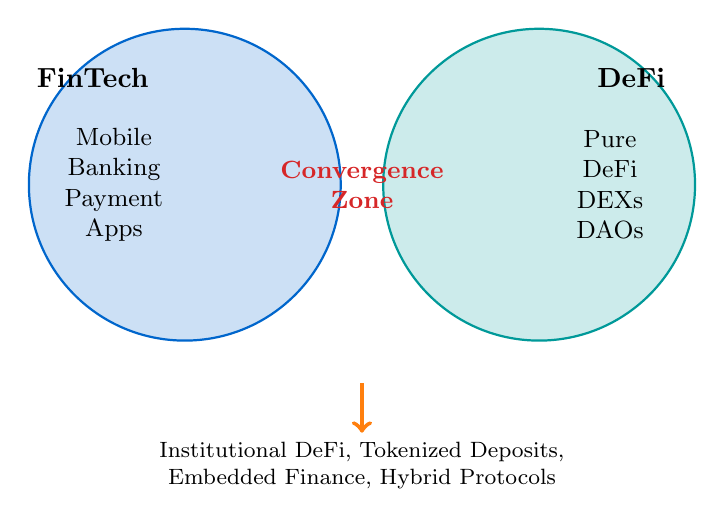
\begin{tikzpicture}[scale=0.9]
% Left circle - FinTech
\draw[thick, dfblue, fill=dfblue!20] (-2.5,0) circle (2.2cm);
\node[font=\bfseries] at (-3.8,1.5) {FinTech};

% Right circle - DeFi
\draw[thick, dfteal, fill=dfteal!20] (2.5,0) circle (2.2cm);
\node[font=\bfseries] at (3.8,1.5) {DeFi};

% Overlap region
\begin{scope}
\clip (-2.5,0) circle (2.2cm);
\fill[dforange!40] (2.5,0) circle (2.2cm);
\end{scope}

% Labels
\node[align=center, font=\small] at (-3.5,0) {Mobile\\Banking\\Payment\\Apps};
\node[align=center, font=\small] at (3.5,0) {Pure\\DeFi\\DEXs\\DAOs};
\node[align=center, font=\small\bfseries, text=dfred] at (0,0) {Convergence\\Zone};

% Arrow below
\draw[->, ultra thick, dforange] (0,-2.8) -- (0,-3.5);
\node[below, font=\footnotesize, align=center] at (0,-3.5) {Institutional DeFi, Tokenized Deposits,\\Embedded Finance, Hybrid Protocols};
\end{tikzpicture}
\end{center}
\end{frame}

% ---------------------------------------------------------------------
\begin{frame}{Why Is Convergence Happening?}
\begin{columns}[T]
\begin{column}{0.48\textwidth}
\textbf{FinTech $\rightarrow$ DeFi:}
\begin{itemize}
\item Cost efficiency (24/7 settlement)
\item Yield opportunities (staking, lending)
\item Programmable money features
\item Customer demand for crypto
\item Competitive pressure
\end{itemize}

\vspace{0.3cm}
\textbf{Examples:}
\begin{itemize}
\item PayPal integrating crypto
\item Robinhood listing tokens
\item Visa settling in USDC
\end{itemize}
\end{column}
\begin{column}{0.48\textwidth}
\textbf{DeFi $\rightarrow$ FinTech:}
\begin{itemize}
\item Regulatory survival
\item Institutional capital access
\item User experience expectations
\item Fiat on/off ramps
\item Compliance requirements
\end{itemize}

\vspace{0.3cm}
\textbf{Examples:}
\begin{itemize}
\item Aave Arc (permissioned pools; limited adoption so far)
\item Circle (regulated stablecoin)
\item Coinbase (public company, licensed)
\end{itemize}
\end{column}
\end{columns}
\end{frame}

% ---------------------------------------------------------------------
\begin{frame}{Convergence Example 1: Institutional DeFi}
\begin{block}{Definition}
DeFi protocols or pools designed for institutions with KYC/AML (Know Your Customer / Anti-Money Laundering), permissioned access, and regulatory compliance.
\end{block}

\begin{columns}[T]
\begin{column}{0.48\textwidth}
\textbf{How it works:}
\begin{itemize}
\item Whitelisted wallet addresses
\item Identity verification required
\item Compliance layer on-chain or off-chain
\item Same smart contracts, restricted access
\end{itemize}
\end{column}
\begin{column}{0.48\textwidth}
\textbf{Key examples:}
\begin{itemize}
\item \textbf{Aave Arc}: Permissioned Aave for institutions (adoption has been limited)
\item \textbf{Compound Treasury}: Institutional lending product
\item \textbf{Maple Finance}: Institutional credit pools
\item \textbf{Centrifuge}: Real-world asset financing
\end{itemize}
\end{column}
\end{columns}

\vspace{0.3cm}
\begin{alertblock}{Key Insight}
Same DeFi rails, different access model. The technology doesn't change; the \emph{governance layer} does.
\end{alertblock}
\end{frame}

% ---------------------------------------------------------------------
\begin{frame}{Convergence Example 2: Tokenized Deposits}
\begin{block}{Definition}
Bank deposits represented as tokens on a blockchain, combining bank liability with blockchain programmability.
\end{block}

\begin{center}
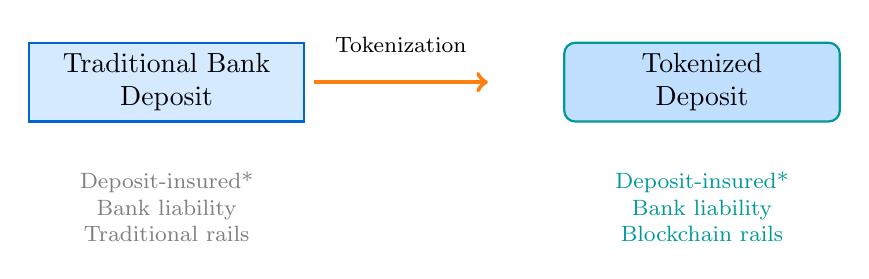
\begin{tikzpicture}[scale=0.85]
% Traditional deposit
\node[process, minimum width=3.5cm, align=center] (bank) at (-4,0) {Traditional Bank\\Deposit};

% Arrow
\draw[->, ultra thick, dforange] (-1.8,0) -- (0.8,0);
\node[above, font=\footnotesize] at (-0.5,0.3) {Tokenization};

% Tokenized deposit
\node[blockchain, minimum width=3.5cm, align=center] (token) at (4,0) {Tokenized\\Deposit};

% Properties below
\node[below, font=\footnotesize, align=center, text=dfgray] at (-4,-1.2) {Deposit-insured*\\Bank liability\\Traditional rails};
\node[below, font=\footnotesize, align=center, text=dfteal] at (4,-1.2) {Deposit-insured*\\Bank liability\\Blockchain rails};
\end{tikzpicture}
\end{center}

\textbf{Key players:} JPMorgan (JPM Coin), Citi, Wells Fargo, Societe Generale

\textbf{Difference from stablecoins:} Tokenized deposits are \emph{bank liabilities}, not claims on reserves held by a separate issuer.

\vspace{1mm}
{\scriptsize *Deposit insurance varies by jurisdiction: FDIC (US), FSCS (UK), Einlagensicherung (EU/Germany). Coverage limits differ.}
\end{frame}

% ---------------------------------------------------------------------
\begin{frame}{Convergence Example 3: Embedded Finance}
\begin{block}{Definition}
Financial services seamlessly integrated into non-financial platforms and workflows.
\end{block}

\begin{columns}[T]
\begin{column}{0.55\textwidth}
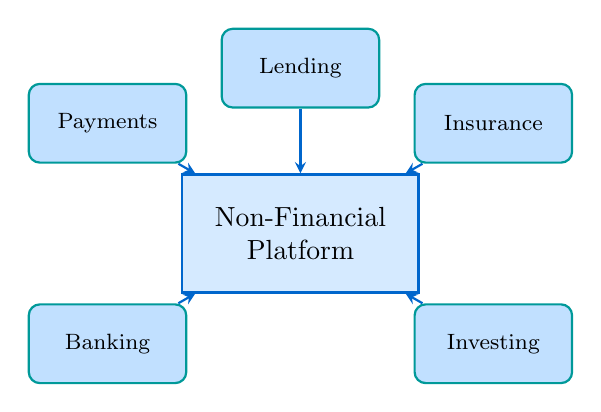
\begin{tikzpicture}[scale=0.7]
% Central platform
\node[process, minimum width=3cm, minimum height=1.5cm, align=center] (platform) at (0,0) {Non-Financial\\Platform};

% Surrounding services
\node[blockchain, minimum width=2cm, font=\footnotesize] (pay) at (-3.5,2) {Payments};
\node[blockchain, minimum width=2cm, font=\footnotesize] (lend) at (0,3) {Lending};
\node[blockchain, minimum width=2cm, font=\footnotesize] (ins) at (3.5,2) {Insurance};
\node[blockchain, minimum width=2cm, font=\footnotesize] (inv) at (3.5,-2) {Investing};
\node[blockchain, minimum width=2cm, font=\footnotesize] (bank) at (-3.5,-2) {Banking};

% Arrows
\draw[arrow] (pay) -- (platform);
\draw[arrow] (lend) -- (platform);
\draw[arrow] (ins) -- (platform);
\draw[arrow] (inv) -- (platform);
\draw[arrow] (bank) -- (platform);
\end{tikzpicture}
\end{column}
\begin{column}{0.42\textwidth}
\textbf{Examples:}
\begin{itemize}
\item Shopify Capital (e-commerce lending)
\item Uber driver instant pay
\item Klarna / Affirm (buy-now-pay-later)
\item Amazon lending to sellers
\item Tesla insurance
\end{itemize}

\vspace{0.3cm}
\textbf{Crypto angle:}
\begin{itemize}
\item Crypto payouts in apps
\item DeFi yields embedded in wallets
\item NFT financing at checkout
\end{itemize}
\end{column}
\end{columns}
\end{frame}

% ---------------------------------------------------------------------
\begin{frame}{Convergence Example 4: Hybrid Protocols}
\begin{columns}[T]
\begin{column}{0.48\textwidth}
\textbf{What makes them hybrid?}
\begin{itemize}
\item On-chain execution + off-chain compliance
\item Decentralized protocol + centralized governance
\item Crypto assets + real-world assets
\item Permissionless base + permissioned layers
\end{itemize}
\end{column}
\begin{column}{0.48\textwidth}
\textbf{Examples:}
\begin{itemize}
\item \textbf{MakerDAO (now Sky)}: DAI backed by RWA vaults (DAI transitioning to USDS)
\item \textbf{Ondo Finance}: Tokenized treasuries
\item \textbf{Backed Finance}: Tokenized ETFs (Exchange-Traded Funds)
\item \textbf{Goldfinch}: Credit to emerging markets
\end{itemize}
\end{column}
\end{columns}

\vspace{0.5cm}
\begin{exampleblock}{MakerDAO's RWA Strategy (now rebranded as Sky, 2024)}
MakerDAO (now Sky) allocates \$2B+ to real-world assets (US Treasuries, corporate bonds). A ``DeFi'' protocol holding TradFi assets---convergence in action.
\end{exampleblock}
\end{frame}

% ---------------------------------------------------------------------
\begin{frame}{Which Innovations Cross the Divide?}
\begin{center}
\textbf{Framework for Evaluating Convergence Likelihood}
\end{center}

\begin{table}[h]
\centering
\small
\begin{tabular}{lcc}
\toprule
\textbf{Factor} & \textbf{High Likelihood} & \textbf{Low Likelihood} \\
\midrule
Regulatory clarity & Clear path & Fundamental conflict \\
Institutional demand & Strong & Weak/retail-only \\
User experience & Comparable to TradFi & Significantly worse \\
Risk profile & Understood, manageable & Novel, unquantifiable \\
Value proposition & Clear efficiency gain & Ideological appeal only \\
\bottomrule
\end{tabular}
\end{table}

\vspace{0.3cm}
\textbf{Most likely to converge:} Payments, lending, asset tokenization\\
\textbf{Least likely:} Privacy coins, fully anonymous DeFi, unregistered securities
\end{frame}

% ---------------------------------------------------------------------
\begin{frame}{Discussion: The Convergence Trade-offs}
\begin{columns}[T]
\begin{column}{0.48\textwidth}
\begin{alertblock}{What's Lost in Convergence?}
\begin{itemize}
\item Permissionlessness
\item Censorship resistance
\item Privacy/pseudonymity
\item Trustlessness
\item Decentralization purity
\end{itemize}
\end{alertblock}
\end{column}
\begin{column}{0.48\textwidth}
\begin{exampleblock}{What's Gained?}
\begin{itemize}
\item Regulatory acceptance
\item Institutional capital
\item Consumer protection
\item Mainstream adoption
\item Integration with existing systems
\end{itemize}
\end{exampleblock}
\end{column}
\end{columns}

\vspace{0.5cm}
\begin{block}{Discussion Questions}
\begin{enumerate}
\item Is ``permissioned DeFi'' still DeFi?
\item Will the permissionless layer survive alongside the permissioned one?
\item Who benefits most from convergence?
\end{enumerate}
\end{block}
\end{frame}

% =====================================================================
%                    SECTION 6.2: AI AND DIGITAL FINANCE
% =====================================================================
\section{6.2 AI and Digital Finance}

% ---------------------------------------------------------------------
\begin{frame}{AI in Finance: The Landscape}
\begin{center}
\begin{tikzpicture}[scale=0.8]
% Central AI node
\node[aibox, minimum width=3cm, minimum height=1.5cm, font=\bfseries] (ai) at (0,0) {AI in Finance};

% Applications around
\node[process, font=\footnotesize, minimum width=2.5cm] (robo) at (-5,2) {Robo-Advisory};
\node[process, font=\footnotesize, minimum width=2.5cm] (fraud) at (0,3) {Fraud Detection};
\node[process, font=\footnotesize, minimum width=2.5cm] (credit) at (5,2) {Credit Scoring};
\node[process, font=\footnotesize, minimum width=2.5cm] (trade) at (5,-2) {Algorithmic Trading};
\node[process, font=\footnotesize, minimum width=2.5cm] (risk) at (0,-3) {Risk Management};
\node[process, font=\footnotesize, minimum width=2.5cm] (nlp) at (-5,-2) {NLP/Chatbots};

% Connections
\draw[arrow, dfpurple] (ai) -- (robo);
\draw[arrow, dfpurple] (ai) -- (fraud);
\draw[arrow, dfpurple] (ai) -- (credit);
\draw[arrow, dfpurple] (ai) -- (trade);
\draw[arrow, dfpurple] (ai) -- (risk);
\draw[arrow, dfpurple] (ai) -- (nlp);
\end{tikzpicture}
\end{center}
\end{frame}

% ---------------------------------------------------------------------
\begin{frame}{AI Application 1: Robo-Advisory}
\begin{columns}[T]
\begin{column}{0.55\textwidth}
\begin{block}{What Is It?}
Automated investment management using algorithms to construct, monitor, and rebalance portfolios based on client goals and risk tolerance.
\end{block}

\textbf{How it works:}
\begin{enumerate}
\item Client inputs: goals, timeline, risk tolerance
\item Algorithm maps to asset allocation
\item Automated portfolio construction
\item Continuous monitoring and rebalancing
\item Tax-loss harvesting (if applicable)
\end{enumerate}
\end{column}
\begin{column}{0.42\textwidth}
\textbf{Key Players:}
\begin{itemize}
\item Betterment
\item Wealthfront
\item Schwab Intelligent Portfolios
\item Vanguard Digital Advisor
\end{itemize}

\vspace{0.3cm}
\textbf{Scale:}
\begin{itemize}
\item \$1.4T+ AUM globally (2024)
\item Fees: 0.25--0.50\% vs. 1\%+ traditional
\item Growing 20\%+ annually
\end{itemize}
\end{column}
\end{columns}

\bottomnote{See Notebook NB13 for hands-on robo-advisor simulation}
\end{frame}

% ---------------------------------------------------------------------
\begin{frame}{Robo-Advisory: The Math Behind It}
\textbf{Mean-Variance Optimization (Markowitz):}

\textbf{Intuition:} Find the mix of assets that gives the best return for a given level of risk. A cautious investor tilts toward bonds; an aggressive one tilts toward stocks.

\begin{equation}
\min_w \frac{1}{2} w^T \Sigma w - \lambda \mu^T w
\end{equation}
\begin{itemize}
\item $w$ = portfolio weights (how much of each asset)
\item $\Sigma$ = covariance matrix (how assets move together)
\item $\mu$ = expected returns vector (how much each asset is expected to earn)
\item $\lambda$ = risk aversion parameter (higher $=$ more cautious)
\end{itemize}
{\scriptsize (Don't worry about the math---the key idea is balancing risk against return automatically.)}

\vspace{0.3cm}
\textbf{Mapping Risk Tolerance to $\lambda$:}
\begin{table}[h]
\centering
\small
\begin{tabular}{lcc}
\toprule
\textbf{Risk Profile} & \textbf{$\lambda$} & \textbf{Typical Equity \%} \\
\midrule
Conservative & 1--2 & 20--40\% \\
Moderate & 3--5 & 40--60\% \\
Aggressive & 6--10 & 60--90\% \\
\bottomrule
\end{tabular}
\end{table}

\bottomnote{Modern robo-advisors add constraints: factor exposure, ESG filters, tax efficiency}
\end{frame}

% ---------------------------------------------------------------------
\begin{frame}{AI Application 2: Fraud Detection}
\begin{columns}[T]
\begin{column}{0.48\textwidth}
\textbf{Traditional Rules-Based:}
\begin{itemize}
\item If transaction > \$10,000 $\rightarrow$ flag
\item If international + new merchant $\rightarrow$ flag
\item Static thresholds
\item High false positive rate
\item Easily gamed once known
\end{itemize}
\end{column}
\begin{column}{0.48\textwidth}
\textbf{ML-Based Detection:}
\begin{itemize}
\item Learns from historical fraud patterns
\item Dynamic thresholds per user
\item Behavioral biometrics
\item Network analysis
\item Adapts to new attack vectors
\end{itemize}
\end{column}
\end{columns}

\vspace{0.5cm}
\begin{block}{Common ML Approaches}
\begin{itemize}
\item \textbf{Supervised}: Random forests, gradient boosting, neural networks on labeled fraud data
\item \textbf{Unsupervised}: Anomaly detection (isolation forests, autoencoders)
\item \textbf{Graph-based}: Network analysis to detect fraud rings
\end{itemize}
\end{block}
\end{frame}

% ---------------------------------------------------------------------
\begin{frame}{AI Application 3: Credit Scoring}
\begin{columns}[T]
\begin{column}{0.48\textwidth}
\textbf{Traditional FICO:}
\begin{itemize}
\item Payment history (35\%)
\item Amounts owed (30\%)
\item Length of history (15\%)
\item New credit (10\%)
\item Credit mix (10\%)
\end{itemize}

\vspace{0.2cm}
\textbf{Limitations:}
\begin{itemize}
\item ``Credit invisible'' populations
\item Backward-looking only
\item Limited data sources
\end{itemize}
\end{column}
\begin{column}{0.48\textwidth}
\textbf{AI/Alternative Data Scoring:}
\begin{itemize}
\item Bank transaction patterns
\item Utility/rent payment history
\item Employment data
\item Education records
\item Behavioral signals
\item Social connections
\end{itemize}

\vspace{0.2cm}
\textbf{Players:}
\begin{itemize}
\item Upstart, ZestFinance, Lenddo
\item Claims: 75\% fewer defaults at same approval rate
\end{itemize}
\end{column}
\end{columns}
\end{frame}

% ---------------------------------------------------------------------
\begin{frame}{AI Application 4: Algorithmic Trading}
\begin{columns}[T]
\begin{column}{0.55\textwidth}
\textbf{Evolution of Quant Trading:}
\begin{enumerate}
\item \textbf{1980s--90s}: Statistical arbitrage
\item \textbf{2000s}: High-frequency trading
\item \textbf{2010s}: Factor investing at scale
\item \textbf{2020s}: Deep learning, NLP, alternative data
\end{enumerate}

\vspace{0.3cm}
\textbf{Modern AI Trading Signals:}
\begin{itemize}
\item Satellite imagery (parking lots, shipping)
\item Social media sentiment
\item Patent filings, job postings
\item Earnings call NLP analysis
\item Web traffic data
\end{itemize}
\end{column}
\begin{column}{0.42\textwidth}
\begin{alertblock}{Reality Check}
\begin{itemize}
\item Most AI trading strategies don't beat benchmarks net of fees
\item Overfitting is rampant
\item Alpha decays quickly once discovered
\item Data quality issues pervasive
\end{itemize}
\end{alertblock}

\textbf{Institutional players:}\\
Two Sigma, Citadel, Renaissance, DE Shaw
\end{column}
\end{columns}
\end{frame}

% ---------------------------------------------------------------------
\begin{frame}{AI in DeFi: Emerging Applications}
\begin{columns}[T]
\begin{column}{0.48\textwidth}
\textbf{Current Applications:}
\begin{itemize}
\item MEV (Maximal Extractable Value---profit extracted by reordering transactions) bots
\item Liquidation bots
\item Yield farming optimizers
\item Portfolio rebalancing agents
\item Smart contract auditing
\end{itemize}
\end{column}
\begin{column}{0.48\textwidth}
\textbf{Emerging/Experimental:}
\begin{itemize}
\item AI-managed DAOs
\item Autonomous trading agents
\item On-chain ML inference
\item LLM-powered governance
\item AI agents holding wallets
\end{itemize}
\end{column}
\end{columns}

\vspace{0.5cm}
\begin{exampleblock}{Example: Yearn Finance}
Yearn uses algorithms to automatically move deposits between yield strategies, optimizing for the highest risk-adjusted returns. Not ``AI'' in the deep learning sense, but algorithmic automation of DeFi.
\end{exampleblock}
\end{frame}

% ---------------------------------------------------------------------
\begin{frame}{AI Risks in Finance: Model Opacity}
\begin{block}{The Black Box Problem}
Complex ML models (neural networks, gradient boosting) often cannot explain \emph{why} they make specific predictions. This creates regulatory and ethical challenges.
\end{block}

\begin{columns}[T]
\begin{column}{0.48\textwidth}
\textbf{Why It Matters:}
\begin{itemize}
\item Regulatory requirements (ECOA, GDPR)
\item Right to explanation for credit denials
\item Model risk management
\item Debugging and improvement
\item Trust and accountability
\end{itemize}
\end{column}
\begin{column}{0.48\textwidth}
\textbf{Mitigation Approaches:}
\begin{itemize}
\item Interpretable models (logistic regression)
\item SHAP/LIME explanations (methods that attribute a prediction to individual input features)
\item Surrogate models
\item Feature importance analysis
\item Regulatory sandboxes
\end{itemize}
\end{column}
\end{columns}

\vspace{0.3cm}
\centering
\textbf{Tension:} More complex models $\rightarrow$ better predictions $\rightarrow$ less interpretability
\end{frame}

% ---------------------------------------------------------------------
\begin{frame}{AI Risks in Finance: Adversarial Attacks}
\begin{block}{Definition}
Deliberately crafted inputs designed to fool ML models while appearing normal to humans.
\end{block}

\begin{columns}[T]
\begin{column}{0.48\textwidth}
\textbf{Finance-Specific Threats:}
\begin{itemize}
\item \textbf{Credit fraud}: Manipulate application to get approval
\item \textbf{Trading}: Poison training data with fake signals
\item \textbf{KYC bypass}: Adversarial images for identity verification
\item \textbf{Spam}: Evade NLP-based filters
\end{itemize}
\end{column}
\begin{column}{0.48\textwidth}
\textbf{Example: Credit Application}
\begin{itemize}
\item Attacker knows model features
\item Slightly modifies spending patterns
\item Opens strategic accounts
\item Model sees ``good'' applicant
\item Fraud not detected until default
\end{itemize}
\end{column}
\end{columns}

\vspace{0.3cm}
\begin{alertblock}{Deepfake Fraud}
AI-generated voice/video for social engineering attacks. A CFO ``calls'' to authorize a wire transfer---but it's a deepfake. Losses in the tens of millions already documented.
\end{alertblock}
\end{frame}

% ---------------------------------------------------------------------
\begin{frame}{AI Risks: Systemic and Concentration}
\begin{columns}[T]
\begin{column}{0.48\textwidth}
\textbf{Herding Risk:}
\begin{itemize}
\item Many firms use similar models
\item Trained on same data
\item Similar predictions $\rightarrow$ same trades
\item Amplifies market moves
\item Flash crashes
\end{itemize}

\vspace{0.3cm}
\textbf{Historical Example:}\\
August 2007 quant meltdown---many funds used similar factor models, simultaneous deleveraging.
\end{column}
\begin{column}{0.48\textwidth}
\textbf{Concentration Risk:}
\begin{itemize}
\item Few dominant AI providers
\item Cloud infrastructure concentration
\item Model monoculture
\item Single points of failure
\end{itemize}

\vspace{0.3cm}
\textbf{Regulatory Response:}
\begin{itemize}
\item EU AI Act (risk classification)
\item Fed/OCC model risk guidance
\item Explainability requirements
\end{itemize}
\end{column}
\end{columns}
\end{frame}

% ---------------------------------------------------------------------
\begin{frame}{AI Claims: A Critical Evaluation Framework}
\textbf{When you hear ``AI will disrupt X in finance,'' ask:}

\begin{enumerate}
\item \textbf{What's the benchmark?} Is AI actually better than existing methods, or just newer?
\item \textbf{Is there enough data?} ML needs large, clean datasets. Rare events (like financial crises) are hard to learn from.
\item \textbf{Is the environment stationary?} Financial markets change; models trained on past data may fail.
\item \textbf{What are the feedback loops?} If everyone uses the same AI, does it still work?
\item \textbf{What's the adversarial dynamic?} Are there incentives to game the model?
\item \textbf{What's the regulatory status?} Can this legally be deployed?
\end{enumerate}

\vspace{0.3cm}
\begin{alertblock}{Healthy Skepticism}
Most AI finance claims are overhyped. Demand evidence: backtests (with proper methodology), out-of-sample performance, real-world deployments.
\end{alertblock}
\end{frame}

% ---------------------------------------------------------------------
\begin{frame}{Hands-On: Robo-Advisor Simulation (NB13)}
\textbf{What you'll do in the notebook:}
\begin{enumerate}
\item Load historical return data for major asset classes
\item Implement mean-variance optimization
\item Map risk tolerance scores to portfolio allocations
\item Visualize efficient frontier
\item Simulate portfolio performance under different risk profiles
\item Add constraints (position limits, ESG filters)
\end{enumerate}

\vspace{0.3cm}
\begin{block}{Key Learning Objectives}
\begin{itemize}
\item Understand how robo-advisors translate preferences to portfolios
\item See the math behind automated investing
\item Recognize the assumptions and limitations
\end{itemize}
\end{block}

\bottomnote{Notebook: NB13\_Robo\_Advisor\_Simulation.ipynb}
\end{frame}

% =====================================================================
%         SECTION 6.3: BUILDING YOUR DIGITAL FINANCE WORLDVIEW
% =====================================================================
\section{6.3 Building Your Digital Finance Worldview}

% ---------------------------------------------------------------------
\begin{frame}{The Challenge of Permanent Knowledge}
\begin{columns}[T]
\begin{column}{0.48\textwidth}
\textbf{What Changes Rapidly:}
\begin{itemize}
\item Specific protocols and platforms
\item Token prices and market caps
\item Regulatory stance by jurisdiction
\item Leading companies and projects
\item Technical implementation details
\end{itemize}
\end{column}
\begin{column}{0.48\textwidth}
\textbf{What's More Durable:}
\begin{itemize}
\item Economic first principles
\item Security vs. convenience tradeoffs
\item Decentralization spectrum
\item Regulatory logic and goals
\item Human behavior patterns
\end{itemize}
\end{column}
\end{columns}

\vspace{0.5cm}
\begin{block}{Goal for Today}
Give you a \textbf{framework}---not facts that will become outdated, but a way of thinking that remains useful for years.
\end{block}
\end{frame}

% ---------------------------------------------------------------------
\begin{frame}{The Digital Finance Innovation Scorecard}
\begin{center}
\textbf{Six Questions for Any Digital Finance Innovation}
\end{center}

\begin{enumerate}
\item \textbf{PROBLEM}: What real problem does this solve, and for whom?
\item \textbf{MECHANISM}: How does it actually work (technically and economically)?
\item \textbf{TRADEOFFS}: What are the key tradeoffs and design choices?
\item \textbf{RISKS}: What could go wrong (technical, economic, regulatory)?
\item \textbf{REGULATORY STATUS}: Where does it fit in the regulatory landscape?
\item \textbf{WHO BENEFITS}: Who captures value, and who bears costs?
\end{enumerate}

\vspace{0.3cm}
\begin{exampleblock}{Design Principle}
These questions work whether you're evaluating Bitcoin in 2009, DeFi in 2020, or whatever comes next in 2030.
\end{exampleblock}
\end{frame}

% ---------------------------------------------------------------------
\begin{frame}{Question 1: PROBLEM}
\begin{block}{Key Sub-Questions}
\begin{itemize}
\item What existing pain point does this address?
\item Who has this problem? (Individuals, businesses, institutions?)
\item How big is the problem? (Market size, frequency, severity)
\item How is it solved today, and why is that solution inadequate?
\item Is the problem real, or is this a ``solution looking for a problem''?
\end{itemize}
\end{block}

\vspace{0.3cm}
\textbf{Red Flags:}
\begin{itemize}
\item Vague problem statements (``revolutionize finance'')
\item No clear user with an urgent need
\item The problem is already well-solved by existing technology
\item Solving a problem only crypto enthusiasts have
\end{itemize}
\end{frame}

% ---------------------------------------------------------------------
\begin{frame}{Question 2: MECHANISM}
\begin{block}{Key Sub-Questions}
\begin{itemize}
\item What is the technical architecture? (Blockchain, centralized, hybrid?)
\item What are the core smart contracts or algorithms?
\item What are the economic incentives that make it function?
\item What assumptions must hold for it to work?
\item What are the dependencies? (Oracles, other protocols, infrastructure)
\end{itemize}
\end{block}

\vspace{0.3cm}
\textbf{Red Flags:}
\begin{itemize}
\item Hand-wavy technical explanations
\item Unsustainable economic incentives (where does the yield come from?)
\item Critical dependencies on single points of failure
\item Complexity without clear purpose
\end{itemize}
\end{frame}

% ---------------------------------------------------------------------
\begin{frame}{Question 3: TRADEOFFS}
\begin{columns}[T]
\begin{column}{0.48\textwidth}
\textbf{Common Tradeoff Dimensions:}
\begin{itemize}
\item Decentralization vs. Efficiency
\item Security vs. Usability
\item Privacy vs. Compliance
\item Innovation vs. Stability
\item Permissionless vs. Permissioned
\item Scalability vs. Security
\end{itemize}
\end{column}
\begin{column}{0.48\textwidth}
\textbf{Key Sub-Questions:}
\begin{itemize}
\item Where does this sit on the spectrum?
\item What was explicitly sacrificed for what gain?
\item Are the tradeoffs appropriate for the use case?
\item Are the tradeoffs honestly communicated?
\end{itemize}
\end{column}
\end{columns}

\vspace{0.3cm}
\begin{alertblock}{No Free Lunch}
Every design choice involves tradeoffs. Be skeptical of claims that offer everything with no downsides.
\end{alertblock}
\end{frame}

% ---------------------------------------------------------------------
\begin{frame}{Question 4: RISKS}
\begin{columns}[T]
\begin{column}{0.32\textwidth}
\textbf{Technical Risks:}
\begin{itemize}
\item Smart contract bugs
\item Oracle failures
\item Scalability limits
\item Key management
\item Dependency risks
\end{itemize}
\end{column}
\begin{column}{0.32\textwidth}
\textbf{Economic Risks:}
\begin{itemize}
\item Death spirals
\item Liquidity crises
\item Incentive misalignment
\item Bank runs
\item Market manipulation
\end{itemize}
\end{column}
\begin{column}{0.32\textwidth}
\textbf{Regulatory Risks:}
\begin{itemize}
\item Securities classification
\item Licensing requirements
\item Enforcement actions
\item Cross-border issues
\item Changing rules
\end{itemize}
\end{column}
\end{columns}

\vspace{0.5cm}
\textbf{Risk Assessment Questions:}
\begin{itemize}
\item What's the worst-case scenario?
\item Has something similar failed before? Why?
\item What's the attack surface?
\end{itemize}
\end{frame}

% ---------------------------------------------------------------------
\begin{frame}{Question 5: REGULATORY STATUS}
\begin{block}{Key Sub-Questions}
\begin{itemize}
\item Is this a security, commodity, currency, or something else?
\item Which regulators have jurisdiction? (SEC, CFTC, FinCEN, state, international)
\item Has there been regulatory guidance or enforcement?
\item What's the compliance strategy? (Licensed, avoiding jurisdiction, fighting)
\item How might regulation evolve?
\end{itemize}
\end{block}

\vspace{0.3cm}
\textbf{Regulatory Classification Matters:}
\begin{table}[h]
\centering
\footnotesize
\begin{tabular}{ll}
\toprule
\textbf{If classified as...} & \textbf{Then...} \\
\midrule
Security & Must register with SEC or use exemptions \\
Commodity & CFTC oversight for derivatives \\
Money transmission & State licenses required \\
Banking product & OCC/Fed/FDIC oversight (US); PRA/FCA (UK); ECB/BaFin (EU) \\
\bottomrule
\end{tabular}
\end{table}
\end{frame}

% ---------------------------------------------------------------------
\begin{frame}{Question 6: WHO BENEFITS}
\begin{block}{Key Sub-Questions}
\begin{itemize}
\item Who captures the economic value? (Founders, investors, users, validators)
\item What are the fee structures and where do fees go?
\item Who bears the risks?
\item Are incentives aligned between stakeholders?
\item Who might be harmed? (Competitors, users of existing systems, society)
\end{itemize}
\end{block}

\vspace{0.3cm}
\begin{columns}[T]
\begin{column}{0.48\textwidth}
\textbf{Value Distribution Analysis:}
\begin{itemize}
\item Token allocation (team, investors, public)
\item Revenue model and fees
\item Governance rights
\end{itemize}
\end{column}
\begin{column}{0.48\textwidth}
\textbf{Red Flags:}
\begin{itemize}
\item Highly concentrated token ownership
\item Misaligned incentives
\item Users bear risk, insiders capture upside
\end{itemize}
\end{column}
\end{columns}
\end{frame}

% ---------------------------------------------------------------------
\begin{frame}{Applying the Framework: Example Analysis}
\begin{center}
\textbf{Quick Scorecard: Stablecoins}
\end{center}

\begin{table}[h]
\centering
\footnotesize
\begin{tabular}{lp{10cm}}
\toprule
\textbf{Question} & \textbf{Analysis} \\
\midrule
PROBLEM & Dollar-denominated value transfer on blockchain; hedging crypto volatility \\
MECHANISM & Varies: fiat-backed (USDC), crypto-backed (DAI), algorithmic (failed: UST) \\
TRADEOFFS & Centralized (USDC) = more stable but censorable; Decentralized (DAI) = more complex \\
RISKS & Reserve quality, depegs, regulatory crackdown, bank runs \\
REGULATORY & Money transmission + potential securities issues; evolving globally \\
WHO BENEFITS & Issuers (interest on reserves), traders (liquidity), DeFi (composability) \\
\bottomrule
\end{tabular}
\end{table}
\end{frame}

% ---------------------------------------------------------------------
\begin{frame}{Capstone Exercise: Innovation Scorecard (NB14)}
\textbf{What you'll do in the notebook:}
\begin{enumerate}
\item Select a digital finance innovation to evaluate
\item Work through each of the six questions systematically
\item Score the innovation on key dimensions
\item Visualize your analysis (radar chart)
\item Compare with classmates' analyses
\end{enumerate}

\vspace{0.3cm}
\begin{block}{Suggested Innovations to Analyze}
\begin{multicols}{2}
\begin{itemize}
\item Real-world asset tokenization
\item Decentralized identity
\item AI-managed portfolios
\item Central Bank Digital Currencies
\item Prediction markets
\item Decentralized insurance
\item Tokenized treasuries
\item Cross-chain bridges
\end{itemize}
\end{multicols}
\end{block}

\bottomnote{Notebook: NB14\_Innovation\_Scorecard.ipynb}
\end{frame}

% ---------------------------------------------------------------------
\begin{frame}{Synthesis: The Lenses We've Developed}
\begin{center}
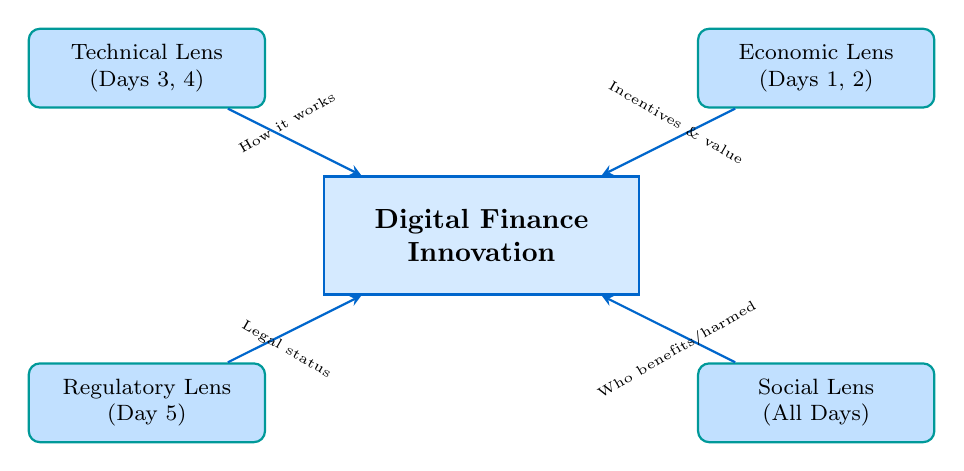
\begin{tikzpicture}[scale=0.85]
% Central node
\node[process, minimum width=4cm, minimum height=1.5cm, font=\bfseries, align=center] (center) at (0,0) {Digital Finance\\Innovation};

% Four lenses
\node[blockchain, minimum width=3cm, font=\footnotesize, align=center] (tech) at (-5,2.5) {Technical Lens\\(Days 3, 4)};
\node[blockchain, minimum width=3cm, font=\footnotesize, align=center] (econ) at (5,2.5) {Economic Lens\\(Days 1, 2)};
\node[blockchain, minimum width=3cm, font=\footnotesize, align=center] (reg) at (-5,-2.5) {Regulatory Lens\\(Day 5)};
\node[blockchain, minimum width=3cm, font=\footnotesize, align=center] (social) at (5,-2.5) {Social Lens\\(All Days)};

% Arrows
\draw[arrow] (tech) -- (center);
\draw[arrow] (econ) -- (center);
\draw[arrow] (reg) -- (center);
\draw[arrow] (social) -- (center);

% Labels on arrows
\node[font=\tiny, above, rotate=30] at (-2.8,1.5) {How it works};
\node[font=\tiny, above, rotate=-30] at (2.8,1.5) {Incentives \& value};
\node[font=\tiny, below, rotate=-30] at (-2.8,-1.5) {Legal status};
\node[font=\tiny, below, rotate=30] at (2.8,-1.5) {Who benefits/harmed};
\end{tikzpicture}
\end{center}

\textbf{Complete analysis requires all four lenses.}
\end{frame}

% =====================================================================
%                    SECTION 6.4: WHAT'S NEXT?
% =====================================================================
\section{6.4 What's Next?}

% ---------------------------------------------------------------------
\begin{frame}{The Genuinely Open Questions}
\begin{block}{These questions will shape the next decade of digital finance:}
\end{block}

\begin{enumerate}
\item \textbf{Interoperability}: Will we see one dominant chain, many chains, or seamless cross-chain?
\item \textbf{CBDC vs. Private Money}: Will central bank digital currencies dominate, or coexist with stablecoins?
\item \textbf{Decentralized Identity}: Will blockchain-based identity systems achieve adoption?
\item \textbf{Quantum Threats}: How will cryptography adapt to quantum computing?
\item \textbf{AI Autonomy}: Will AI agents hold assets and transact independently?
\item \textbf{Regulatory Equilibrium}: Where will global regulation settle?
\item \textbf{The Future of Money}: What \emph{is} money in 2035?
\end{enumerate}
\end{frame}

% ---------------------------------------------------------------------
\begin{frame}{Open Question: Interoperability}
\begin{columns}[T]
\begin{column}{0.48\textwidth}
\textbf{Current State:}
\begin{itemize}
\item Multiple Layer 1 chains (Ethereum, Solana, etc.)
\item Multiple Layer 2s (Arbitrum, Optimism, Base)
\item Fragmented liquidity
\item Bridge vulnerabilities (\$2B+ hacked)
\item Poor user experience
\end{itemize}
\end{column}
\begin{column}{0.48\textwidth}
\textbf{Possible Futures:}
\begin{itemize}
\item \textbf{One chain wins}: Network effects concentrate
\item \textbf{Chain abstraction}: Users don't know/care which chain
\item \textbf{Specialized chains}: Different chains for different uses
\item \textbf{Traditional wins}: Banks don't need public chains
\end{itemize}
\end{column}
\end{columns}

\vspace{0.3cm}
\begin{block}{Discussion Question}
Is the future of blockchain ``one chain to rule them all'' or an interoperable multi-chain world? What are the arguments for each?
\end{block}
\end{frame}

% ---------------------------------------------------------------------
\begin{frame}{Open Question: CBDCs vs. Private Digital Money}
\begin{columns}[T]
\begin{column}{0.48\textwidth}
\textbf{Arguments for CBDCs:}
\begin{itemize}
\item Central bank backing = safe
\item Monetary policy transmission
\item Financial inclusion
\item Reduced settlement risk
\item Programmable policy tools
\end{itemize}

\vspace{0.2cm}
\textbf{Status:} 130+ countries exploring; China, Nigeria, Bahamas live
\end{column}
\begin{column}{0.48\textwidth}
\textbf{Arguments for Private Money:}
\begin{itemize}
\item Innovation at the edge
\item Competition improves quality
\item Privacy from government
\item Borderless by design
\item Decentralization values
\end{itemize}

\vspace{0.2cm}
\textbf{Stablecoin market cap:} $\sim$\$230B+ (as of early 2025; check CoinGecko for current figures)
\end{column}
\end{columns}

\vspace{0.3cm}
\begin{alertblock}{The Coexistence Hypothesis}
Most likely: CBDCs for domestic retail, regulated stablecoins for crypto/DeFi, and continued competition between payment systems.
\end{alertblock}
\end{frame}

% ---------------------------------------------------------------------
\begin{frame}{Open Question: Decentralized Identity}
\begin{block}{The Problem}
Online identity today is fragmented, insecure, and controlled by platforms. Can blockchain fix this?
\end{block}

\begin{columns}[T]
\begin{column}{0.48\textwidth}
\textbf{DID/SSI Vision:}
\begin{itemize}
\item Self-sovereign identity
\item User controls their data
\item Selective disclosure
\item Portable across platforms
\item Verifiable credentials
\end{itemize}
\end{column}
\begin{column}{0.48\textwidth}
\textbf{Challenges:}
\begin{itemize}
\item Key management for everyday users
\item Recovery when keys lost
\item Adoption chicken-and-egg
\item Regulatory acceptance
\item Competition from Big Tech
\end{itemize}
\end{column}
\end{columns}

\vspace{0.3cm}
\textbf{Watch:} EU eIDAS 2.0, Worldcoin, ENS, Soulbound tokens, Polygon ID
\end{frame}

% ---------------------------------------------------------------------
\begin{frame}{Open Question: Quantum Computing Threats}
\begin{columns}[T]
\begin{column}{0.48\textwidth}
\textbf{What's at Risk:}
\begin{itemize}
\item ECDSA (Elliptic Curve Digital Signature Algorithm---used by Bitcoin, Ethereum)
\item RSA encryption (widely used public-key cryptosystem)
\item Current digital signatures
\item Potentially: all historical transactions
\end{itemize}

\vspace{0.2cm}
\textbf{``Harvest Now, Decrypt Later''}: Adversaries may be storing encrypted data to break when quantum arrives.
\end{column}
\begin{column}{0.48\textwidth}
\textbf{Mitigation Paths:}
\begin{itemize}
\item Post-quantum cryptography (NIST standards)
\item Hash-based signatures (already quantum-resistant)
\item Migration plans for blockchains
\item Timeline uncertainty (10--30 years?)
\end{itemize}

\vspace{0.2cm}
\textbf{Good news:} Most blockchain systems can upgrade signature schemes.
\end{column}
\end{columns}
\end{frame}

% ---------------------------------------------------------------------
\begin{frame}{Open Question: AI Agents in Finance}
\begin{block}{The Emerging Possibility}
AI agents that autonomously hold assets, execute transactions, and make financial decisions.
\end{block}

\begin{columns}[T]
\begin{column}{0.48\textwidth}
\textbf{Current Reality:}
\begin{itemize}
\item Bots executing programmed strategies
\item Human-supervised automation
\item Narrow, well-defined tasks
\end{itemize}
\end{column}
\begin{column}{0.48\textwidth}
\textbf{Speculative Future:}
\begin{itemize}
\item AI agents with their own wallets
\item Agent-to-agent transactions
\item AI-managed DAOs
\item Autonomous economic actors
\end{itemize}
\end{column}
\end{columns}

\vspace{0.3cm}
\begin{alertblock}{Legal and Ethical Questions}
Can an AI agent be a legal entity? Who is liable when an AI makes a bad financial decision? How do we prevent AI agents from being used for money laundering?
\end{alertblock}
\end{frame}

% ---------------------------------------------------------------------
\begin{frame}{Open Question: The Future of Money}
\begin{center}
\textbf{What will ``money'' mean in 2035?}
\end{center}

\begin{columns}[T]
\begin{column}{0.48\textwidth}
\textbf{Continuity View:}
\begin{itemize}
\item Central banks remain dominant
\item Digital but still state-controlled
\item Private innovation at the margins
\item Regulation tightens
\item Status quo with better UX
\end{itemize}
\end{column}
\begin{column}{0.48\textwidth}
\textbf{Disruption View:}
\begin{itemize}
\item Multiple competing currencies
\item Programmable money standard
\item Algorithmic monetary policy
\item Borderless by default
\item Fundamental restructuring
\end{itemize}
\end{column}
\end{columns}

\vspace{0.5cm}
\centering
\textbf{The only certainty: more change is coming.}
\end{frame}

% ---------------------------------------------------------------------
\begin{frame}{Group Discussion: Your Hypotheses}
\begin{block}{Instructions}
Form groups of 3--4. Each group picks one open question and develops a hypothesis about how it will unfold over the next decade. Be prepared to defend your view.
\end{block}

\vspace{0.3cm}
\textbf{Structure your hypothesis:}
\begin{enumerate}
\item \textbf{Claim}: What do you think will happen?
\item \textbf{Evidence}: What current trends support this?
\item \textbf{Assumptions}: What must be true for your prediction to hold?
\item \textbf{Risks to thesis}: What could prove you wrong?
\item \textbf{Implications}: If you're right, what follows?
\end{enumerate}
\end{frame}

% =====================================================================
%                    COURSE SUMMARY
% =====================================================================
\section{Course Summary}

% ---------------------------------------------------------------------
\begin{frame}{What We Covered: The Six-Day Journey}
\begin{table}[h]
\centering
\footnotesize
\begin{tabular}{clp{8cm}}
\toprule
\textbf{Day} & \textbf{Theme} & \textbf{Key Takeaways} \\
\midrule
1 & Foundations & What is money; financial system pain points; FinTech vs.\ DeFi framing; landscape overview \\
2 & Digital Finance & Digital payments; API economy \& BaaS; data-driven finance; platform economics \\
3 & Blockchain & Cryptographic building blocks; blockchain mechanics; wallets \& transactions; Bitcoin vs.\ Ethereum \\
4 & Smart Contracts \& DeFi & Smart contracts; DeFi primitives (AMMs, lending); stablecoins; tokenization \& CBDCs \\
5 & Risks \& Regulation & What goes wrong (hacks, failures); regulatory landscapes; DAO governance; privacy \& inclusion \\
6 & Future & Convergence thesis; AI in digital finance; synthesis framework; what's next \\
\bottomrule
\end{tabular}
\end{table}
\end{frame}

% ---------------------------------------------------------------------
\begin{frame}{Key Competencies You've Developed}
\begin{columns}[T]
\begin{column}{0.48\textwidth}
\textbf{Technical Understanding:}
\begin{itemize}
\item How blockchains achieve consensus
\item Smart contract mechanics
\item DeFi protocol design
\item Security considerations
\end{itemize}

\vspace{0.3cm}
\textbf{Economic Reasoning:}
\begin{itemize}
\item Incentive analysis
\item Market structure effects
\item Risk-return tradeoffs
\item Value capture dynamics
\end{itemize}
\end{column}
\begin{column}{0.48\textwidth}
\textbf{Regulatory Awareness:}
\begin{itemize}
\item Classification frameworks
\item Jurisdictional differences
\item Compliance requirements
\item Regulatory trajectory
\end{itemize}

\vspace{0.3cm}
\textbf{Critical Evaluation:}
\begin{itemize}
\item Separating hype from substance
\item Identifying risks and tradeoffs
\item Asking the right questions
\item Framework for any innovation
\end{itemize}
\end{column}
\end{columns}
\end{frame}

% ---------------------------------------------------------------------
\begin{frame}{The Durable Lessons}
\begin{enumerate}
\item \textbf{No free lunch}: Every design choice involves tradeoffs. Be skeptical of claims that offer everything.

\item \textbf{Incentives matter}: Understand who profits and how. Follow the money.

\item \textbf{Technology is not enough}: Great tech fails without regulatory clarity, user adoption, and sustainable economics.

\item \textbf{Regulation follows innovation}: The rules will change. Build with regulatory evolution in mind.

\item \textbf{Decentralization is a spectrum}: Most systems are more centralized than marketed. That's not always bad.

\item \textbf{Convergence is coming}: The FinTech-DeFi divide is dissolving. Prepare for hybrid futures.

\item \textbf{Stay curious, stay skeptical}: This field moves fast. Your framework for evaluation matters more than any specific fact.
\end{enumerate}
\end{frame}

% ---------------------------------------------------------------------
\begin{frame}{Resources for Continued Learning}
\begin{columns}[T]
\begin{column}{0.48\textwidth}
\textbf{News and Analysis:}
\begin{itemize}
\item The Block, CoinDesk (crypto)
\item Risk.net, American Banker (TradFi)
\item a16z crypto blog
\item BIS working papers
\end{itemize}

\vspace{0.3cm}
\textbf{Technical Deep Dives:}
\begin{itemize}
\item Ethereum docs
\item DeFi protocol documentation
\item Academic papers (SSRN, NBER)
\end{itemize}
\end{column}
\begin{column}{0.48\textwidth}
\textbf{Regulatory Updates:}
\begin{itemize}
\item SEC, CFTC releases
\item EU MiCA documentation
\item FSB reports
\end{itemize}

\vspace{0.3cm}
\textbf{Communities:}
\begin{itemize}
\item Protocol governance forums
\item Twitter/X crypto finance
\item Academic conferences (AFA, WFA)
\end{itemize}
\end{column}
\end{columns}

\vspace{0.3cm}
\centering
\textbf{The course ends here. Your journey continues.}
\end{frame}

% ---------------------------------------------------------------------
\begin{frame}{Final Reflection}
\begin{center}
\Large
\textbf{``The best way to predict the future\\is to invent it.''}\\[0.5cm]
\normalsize
--- Alan Kay

\vspace{1cm}

You now have the tools to not just observe digital finance,\\
but to \textbf{critically evaluate}, \textbf{thoughtfully participate},\\
and perhaps \textbf{help shape} its future.

\vspace{1cm}

\textbf{Thank you for your engagement throughout the course.}
\end{center}
\end{frame}

% =====================================================================
%                    END
% =====================================================================

\end{document}
